\section{Related work on supervised approaches} \label{hmc}

In this chapter, we present the relevant literature regarding supervised approaches to \acrfull{si}. We focus on the literature regarding \acrfull{hmc}, a problem in machine learning where objects can be assigned an arbitrary number of labels, and where the labels form a hierarchy. It is a specific case of the \acrfull{mlc} problem. The models are trained by feeding them labeled data, which in our case are assignments of subjects to documents.

\acrshort{hmc} has applications in various disciplines other than \acrfull{nlp}, such as in computer vision, for object recognition tasks, or in biomedicine for predicting the function of proteins. Given the popularity in research of these two disciplines, there is a lot of literature regarding \acrshort{hmc}. We start this chapter by introducing \acrshort{hmc}, including its different approaches. We then go over several neural network architectures that we deem suitable for our use case, and present the relevant literature for each of them.

Binary classifiers are not suitable for our use case because our number of subjects is too high: training 2,157 independent binary classifiers would be computationally expensive. We therefore focus on approaches that comprise only one model, which is responsible for computing the assignment probabilities of all subjects. Convolutional models are well suited for our task because of their feature extraction capabilities. We have found such a model in the literature (\cite{gargiulo2019deep}) that is applied to a similar use case. It will be the basis of our implementation. This model is presented in section \ref{hmc_gargiulo}

We will extend the model in two ways. First, we modify the loss function to account for the imbalance between positive and negative labels in multi-label settings \cite{ben2020asymmetric}, as explained in section \ref{hmc_asl}. The second extension is the implementation of the current \acrshort{sota} in \acrshort{hmc}, which only involves adding a layer on top of the model and again modifying the loss function. This extension ensures that the assignment probability output by the model for each subject is at least as high as the probabilities of its descendants in the hierarchy \cite{giunchiglia2020coherent}. The details of this implementation are shown in section \ref{hmc_forward}.

We also present an application of recurrent networks to \acrshort{hmc}. The recurrence is applied to the levels of the subject hierarchy, which increases the efficiency of the model because of the shared weights \cite{wehrmann2018hierarchical}. However, we discard implementing them, as the authors of the recurrent network show in their experiments that it performs worse than the analogous feed-forward network where the weights are not shared across levels.

\subsection{Introduction} \label{problem_intro}

As discussed in chapter \ref{repo_analysis}, the subjects that are currently present in the repositories are not well maintained. 81 \% of all subjects occur only once, i.e. they are only used by one publication. These cannot be used to relate documents. Furthermore, only 5 \% of the subjects are used by more than 3 publications. The poor quality of the subjects decreases the accessibility of the repositories. Each of them contains thousands of documents, and navigating them can be a cumbersome task. Subjects can be a useful tool for finding the desired documents, and also for looking for documents that are related to the ones we are currently reading.

Consider a repository where there is a maintained set of subjects. Each document in the repository is assigned a subset of these subjects, which can be navigated through the document's page in the repository. If a user is currently reading a publication about brain-computer interfacing, and would like to read more about that topic, the user could browse other documents that handle it by clicking on the corresponding subject. Furthermore, if the user has trouble understanding one of the building blocks of the documents, the user can click on the corresponding subject to search for other documents that maybe present that concept in more detail.
\subsection{Binary classifiers}

Binary classifiers address the data imbalance, which results in poor performance down the hierarchy because of lack of training data, by being optimized individually for each label \cite{banerjee2019hierarchical}. However, multi-label scenarios are usually full of dependencies among labels, which independent binary classifiers do not take into account \cite{liu2017deep}. Furthermore, a collection of binary classifiers is only an option when the number of labels doesn't exceed a few hundreds \cite{banerjee2019hierarchical}. This approach is therefore not interesting for our use case, where there are thousands of labels.
\subsection{Convolutional networks} \label{hmc_cnn}

Convolutions were originally designed for image. However, they can also be used on text, to reduce the size of the data while keeping relevant information. Doing so helps with regularization, as the complexity of the data is reduced. \cite{kim2014convolutional} proposed one-dimensional convolutions and pooling for text input, which are now the common approach. We present these operations here, before discussing two relevant implementations of convolutions for \acrshort{hmc} tasks.

\subsubsection{Convolutions for text}

When applied to text, convolutions are usually one-dimensional. In contrast, convolutions are two-dimensional when applied to images. This has to do with the structure of text and images. The words in a text are ordered across one dimension, whereas the pixels of an image are located in a two-dimensional space. Convolutions extract features from multiple word vectors at a time. Therefore, the result doesn't necessarily change the number of vectors; it affects the number of dimensions.

The number of filters is the number of features we want to extract from each word vector, when considering its surroundings. How large the considered context is, is defined by the kernel size. The number of vectors can be ensured to remain constant with padding, which is done in the original implementation. A single convolution receives $k$ one-dimensional vectors of size $n$ and outputs a single one-dimensional vector of size $m$. $k$ is the kernel size, which defines how many words are considered by each convolution, and $m$ is the number of filters (what PyTorch refers to as output channels), which defines how many vectors remain after the convolutional layer.

\subsubsection{Pooling for text}

Pooling is used to reduce the size of the data while keeping the most important information. The original implementation uses the most popular form of pooling, called max-pooling. Max-pooling takes the maximum over each dimension of the data, thus reducing the number of word vectors. Recall that each dimension represents a feature. The kernel size of the pooling layer defines how many word vectors are considered at a time. For instance, if the kernel size is two, the number of vectors is halved, as the maximum value for all dimensions of each pair of word vectors is kept.

\subsubsection{CNN for HMC} \label{hmc_gargiulo}

\cite{gargiulo2019deep} uses a convolutional model and various embedding methods to index medical documents with MeSH subjects, a hierarchical set of 27,775 subjects regarding Medicine and Biology. Their dataset consists of over eleven million documents from PubMed.

Their architecture comprises three stages. In the first stage, the words are replaced by vectors. The authors try different embedding methods, including the pre-trained fasttext vectors and a normalization pipeline that lower-cased and tokenized the texts, as well as removing numbers punctuation signs, numbers and stopwords. The remaining words were then lemmatized. This is not really an embedding method, but does play an important role in the quality of the embeddings. They experimented with five different embedding methods and various combinations of them. They concluded that the normalization pipeline significantly increased the performance of the model, whereas concatenating different embeddings usually decreased the model's accuracy.

The second stage of their architecture, termed \textit{feature extraction module}, consists of two convolutional layers, followed by max-pooling layers, which reduce the dimensionality of the data while hopefully retaining as much information as possible. A dropout layer with 1 \% discard probability ends this stage, as a regularization method. Interestingly, their first max-pooling layer is said to have size 1, meaning that the maximum value is picked for each window of size 1. This of course is useless; the input to the layer is forwarded without any modifications. We have looked in related work for an explanation, but unfortunately couldn't find any. A previous paper of the first author shows a similar convolutional architecture, but where the max-pooling layer has size 2. This is also the case for the second max-pooling layer in this architecture.

The third and final stage of their architecture is where the indexing occurs. It comprises two fully connected layers, where the size of the output layer equals the number of labels. The first layer has a Rectified Linear Unit (ReLU) activation function and the second, a sigmoid function. The second and third stages, which are the actual neural network model, are depicted in figure \ref{fig:gargiulo}. The first convolutional layer receives a matrix with $N$ words, each of $D$ dimensions. The authors chose 400 as the number of words, padding documents with less words and truncating those with more.

\begin{figure}
    \centering
    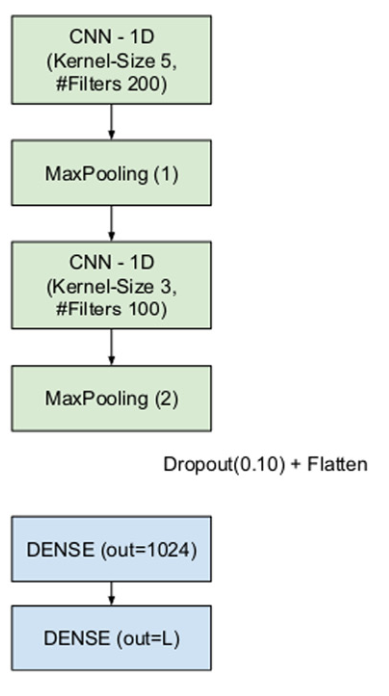
\includegraphics[width=.3\textwidth]{figures/hmc/gargiulo.png}
    \caption{Convolutional architecture for HMC from \cite{gargiulo2019deep}.}
    \label{fig:gargiulo}
\end{figure}

The model is trained with the \acrfull{bce} loss function, which is often used in multi-label settings because each label is treated independently. The model is trained with \acrfull{sgd}, with a mini-batch size of 10, momentum 0.9 and Nesterov accelerated gradients. Besides the comparison of embedding methods, their contribution includes a regularization method, called Hierarchical Label Set Expansion (HLSE), which ensures that if a subject is assigned to a document, its parents are assigned as well. This regularization method reduces the noise in the data, but also increases the complexity of the task, as more labels have to be predicted. However, their experiments conclude that HLSE does increase model accuracy.

\subsection{Feed-forward networks}  \label{hmc_forward}

Feed-forward neural networks are formed by nodes that are connected as a directed acyclic graph (DAG), meaning that there are no cycles. Multi-layer perceptrons, the first kind of neural networks to arise, are a kind of feed-forward networks, where the layers have threshold activation.

\subsubsection{HMC Networks}

\cite{wehrmann2018hierarchical} presents a feed-forward architecture that outperforms previous \acrshort{hmc} approaches for a variety of use cases and datasets. The network comprises one layer per level in the subject hierarchy, each outputting its own local loss. These losses are then added to the global loss, after being weighted. How important local losses are is case-dependent. Therefore, the weight parameter can be adjusted.

Each layer also receives the original input, as shown in figure \ref{fig:hmcn-f}. This allows each layer to associate features from the input to the classes of the hierarchy level it represents. Thus, a layer learns features for a specific level of the subject hierarchy by processing both the original input and the output of the previous layer, i.e. the previous level of the hierarchy. According to the authors, introducing local losses feeds the network with specific local information that would otherwise be ignored, and prevents dead neurons (i.e. neurons with weight and bias close to zero) because of the increased gradient signal, which also accelerates convergence.

As is common in the multi-label setting, the authors have also picked binary cross-entropy as the loss function. Training is controlled by the Adam optimizer and a learning rate of $10^{-3}$. They used ReLU activation functions for all hidden neurons and sigmoid for the output neurons. Batches are normalized and their parameters are dropped out with a probability of 60 \% to avoid overfitting.

\begin{figure}
    \centering
    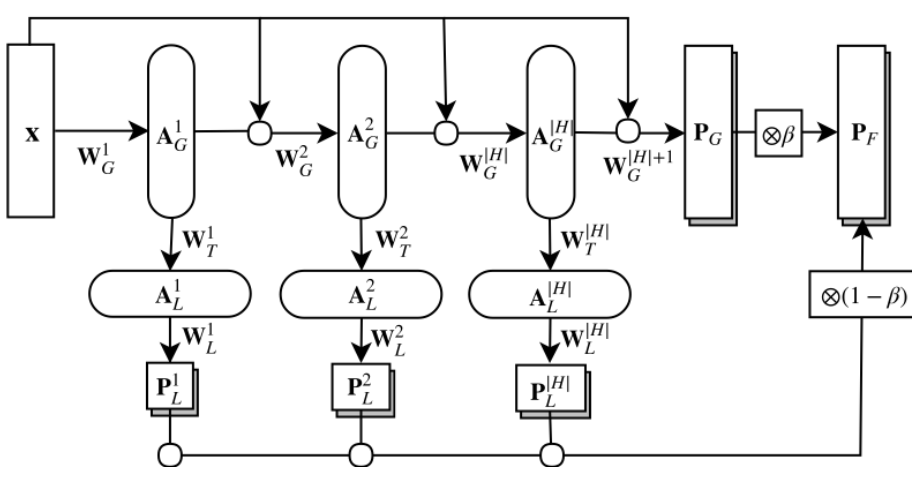
\includegraphics[width=.8\textwidth]{figures/hmc/hmcn-f.png}
    \caption{Architecture of the feed-forward HMC network from \cite{wehrmann2018hierarchical}.}
    \label{fig:hmcn-f}
\end{figure}

\subsubsection{Coherent HMC Networks}

Another feed-forward architecture was proposed in \cite{giunchiglia2020coherent}, which outperformed the architecture presented above in 17 out of 20 datasets, with a much simpler architecture. Instead of introducing local losses for the levels of the hierarchy, this approach enforces the hierarchy on the assignment probabilities by modifying the probabilities of subjects if one of their descendants has higher probability.

For example, if a document is assigned the subject \textit{k-nearest neighbors} with probability $0.7$, the probability of \textit{clustering algorithms} should at least be $0.7$. The authors ensure this is the case by picking for each class the maximum probability between its own probability and the probabilities of its descendants in the hierarchy. Formally, they introduce this constraint in the architecture with an additional layer called \acrfull{mcm}, which, for each subject, picks the maximum probability between its own and that of its descendants. Given a subject $A$ and its descendant $B$, for which a model outputs probabilities $p_A$ and $p_B$, the \acrshort{mcm} outputs the following probabilities for each node:

\begin{align*} 
    & MCM_B = p_B \\ 
    & MCM_A = \max(p_A, MCM_B)
\end{align*}

Their second contribution is a modification of the \acrfull{bce} loss function, which doesn't take into account the dependencies between labels. Their loss function incentivizes the model to respect the subject hierarchy, i.e. that subjects should not be assigned probabilities lower than the probabilities of its descendants. This loss function, called \acrfull{mcl}, can be defined for the two nodes $A$ and $B$ described above as follows:

\begin{align*} 
    & MCL_B = -y_B \ln(MCM_B) - (1 - y_B) \ln(1 - MCM_B) \\ 
    & MCL_A = -y_A \ln(\max(p_A, p_B \cdot y_B)) - (1 - y_A) \ln(1 - MCM_A)
\end{align*}

The loss for the descendant subject $B$ is computed exactly as in the \acrshort{bce} loss function, using $MCM_B$ instead of the model's output $p_B$. Note that $y_A, y_B \in {0, 1}$ are the true labels of the subjects $A$ and $B$ for a given document. The loss for the ancestor subject $A$ differs from the \acrshort{bce} loss in that in the first logarithmic term. In fact, it only changes when the subject $B$ should be assigned to the document (i.e. $y_b = 1$). Then, the loss of its ancestor $A$ takes the max function takes the maximum between $p_A$ and $p_B$ for the first logarithmic term of its loss.

For example, if the descendant subject $B$ had a higher probability than its ancestor $A$ in the model output ($p_B > p_A$) and only $A$ should be assigned to the document ($y_A = 1, y_B = 0$), the \acrshort{bce} loss would wrongly output that $p_B$ should be increased and $p_A$ kept as is. MCL, on the other hand, outputs the right losses, stating that $p_A$ should be increased and $p_B$ decreased, so the hierarchy is not violated.
\subsection{Recurrent networks}

Recurrent neural networks are similar to feed-forward networks, but their nodes do form a cycle, This allows them to exhibit temporal behavior, i.e. they can handle sequential data. They are also characterized by their efficiency, as weights are shared across the layers (which are iterations in the presence of recurrence), making recurrent networks much smaller than feed-forwad networks.

\subsubsection{HMC Networks}

\cite{wehrmann2018hierarchical}, whose feed-forward network we presented above, also proposes a recurrent architecture. The feed-forward architecture already resembles a recurrent network, with each layer having its own input and output, while being sequentially communicated with other layers. Therefore, modifying it to be recurrent is straight forward. Doing so also addresses an issue of the feed-forward network, namely that the number of parameters increases with the number of hierarchy levels. Recurrent networks share weights across layers, therefore having a constant number of weights, regardless of the number of levels in the hierarchy.

The authors used a Long Short-Term Memory (LSTM) architecture for their recurrent network, which already regulates the gradient and thus prevents it from vanishing during the backward pass. The recurrent network was slightly worse than the feed-forward one, but is much smaller in terms of parameters. In one of their experiments, the feed-forward architecture had seven million parameters, whereas the recurrent network had three million. The authors recommend using the recurrent network for hierarchies with many levels, as in such cases the difference in size between the architectures is larger and the minimal gain in performance is not worth the additional complexity.
\subsection{Asymmetric loss function} \label{hmc_asl}

\cite{ben2020asymmetric} addresses the imbalance between positive and negative labels in multi-label settings with an \acrfull{asl} function that dynamically down-weights and hard-thresholds easy negative samples, while also discarding possibly mislabeled samples. Training the state-of-the-art models in computer vision with this loss function significantly outperforms previous methods. On ResNet101, the common architecture used for multi-label classification, the asymmetric loss improves previous results by more than 1 \%. The \acrshort{asl} is also popular for its robustness against noise, as it is better suited for modeling noise in \acrshort{mlc} settings \cite{zhao2021evaluating}. The choice of the loss function plays a key role on how the model handles noise \cite{karimi2020deep}.

\subsubsection{BCE and focal loss}

\acrfull{bce}, the most popular loss function in multi-label classification settings, treats every label the same. For example, in a one-label setting where the model outputs $p=0.7$, if the label is positive ($y=1$), the \acrshort{bce} loss would be $-log(0.7) = 0.4$. If negative ($y=0$), the \acrshort{bce} loss would be $-log(0.3) = 1.2$, i.e. larger than in the other case, as the predicted probability is further away from the true label. The problem with using \acrshort{bce} in a multi-label setting is that most of the true labels for any given input are usually negative. In our case, any document is assigned only a few of the available subjects.

$$ BCE = \frac{1}{K} \sum_{k=1}^K -y_k \cdot \log (p_k) - (1-y_k) \cdot \log (1-p_k) $$

\acrfull{fl} addresses this issue by weighting each label score in a way that model outputs that are further away from their true labels gain more importance, whereas the model outputs that are already close to their targets are weighted down. Returning to the previous example and setting $\gamma=1$, a model output of $0.7$ with a positive true label ($y=1$) would receive a \acrshort{fl} of $-0.3 \cdot log(0.7) = 0.1$, and with a negative label ($y=0$), the \acrshort{fl} would be $-0.7 \cdot log(0.3) = 0.8$.

If we compare the results of both losses, we see that the difference between the results is much larger when using the \acrshort{fl}: they differ by a factor of 8 instead of by a factor of 3. The \acrshort{fl} gives more importance to the model output that was far away from its true label. Thus, the higher the \acrshort{fl} parameter $\gamma$ is set, the larger the difference will be between outputs that are close to their labels and those that are further away. However, setting $\gamma$ too high could remove the gradients from the rare positive samples \cite{ben2020asymmetric}.

$$ FL_\gamma = \frac{1}{K} \sum_{k=1}^K -y_k \cdot (1-p_k)^\gamma \cdot \log (p_k) - (1-y_k)\cdot p_k^\gamma \cdot \log (1-p_k) $$

\subsubsection{Asymmetric loss}

\acrfull{asl} overcomes this issue by decoupling the $\gamma$ parameter for negative and positive true labels, i.e. into $\gamma_-$ and $\gamma_+$, respectively. Setting $\gamma_- > \gamma_+$ emphasizes the contribution of positive samples, while giving less importance to negative samples that are close to their true label. Each of these three loss functions is an extension of the previous one. \acrshort{fl} equals \acrshort{bce} for $\gamma=0$, and \acrshort{asl} equals \acrshort{fl} for $\gamma_- = \gamma_+$.

$$ ASL_{\gamma_-,\gamma_+} = \frac{1}{K} \sum_{k=1}^K -y_k \cdot (1-p_k)^{\gamma_+} \cdot \log (p_k) - (1-y_k)\cdot p_k^{\gamma_-} \cdot \log (1-p_k) $$

The authors also propose using a hard threshold to discard negative samples below it, to further direct the training towards the positive samples. Although improving the performance of the models, this addition increases the complexity of the model, adding another parameter that requires tuning. They also experimented with dynamically tuning the $\gamma$ values, but concluded that doing so hindered the performance of the models. Still, they state this scheme could be useful for novice users.